% Load preamble
\documentclass[../main.tex]{subfiles}

\begin{document}
	\subsection{Úvodný príklad}
	Majme systém, ktorý je určený stavovým opisom \cref{eqn:svlvvPr1SyavovyOpis}. Bloková schéma systému je na \cref{fig:svlvvPr1BlockSchemaSystemu}.
	\begin{equation}
		\begin{gathered}
		\dot{x_1}  =u + \sin(x_1) x_2 \\
		\dot{x_2} = 2x_1 + sin(x_1) \\
		y = x_2
		\end{gathered}
		\label{eqn:svlvvPr1SyavovyOpis}
	\end{equation}
	\begin{figure}[h!]
		\centering
		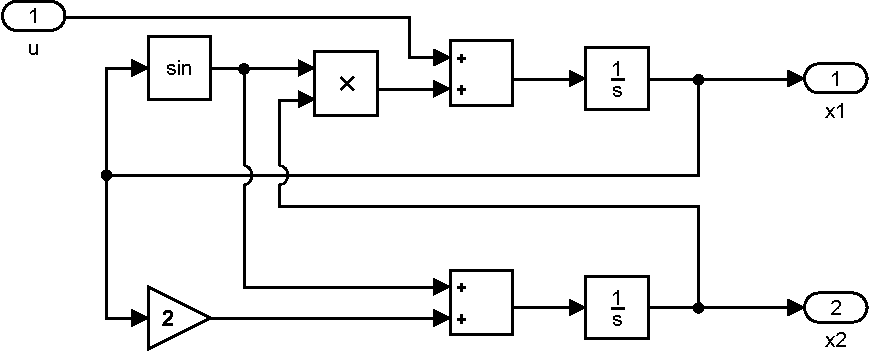
\includegraphics[width=0.8\linewidth]{svlvvPr1/svlvvPr1Sys-crop}
		\caption{Bloková schéma systému z \cref{eqn:svlvvPr1SyavovyOpis}}
		\label{fig:svlvvPr1BlockSchemaSystemu}
	\end{figure}

	Overme teraz, že bod  $x_1 = x_2 = 0$, je rovnovažný bodom systému.
	\begin{equation*}
	\begin{gathered}
	\dot{x_1}|_{x_1 = x_2 = 0}  = \sin(0) 0 = 0 \\
	\dot{x_2}|_{x_1 = x_2 = 0} = 0 + sin(0) = 0 \\
	\end{gathered}
	\label{eqn:svlvvPr1OverenieRB}
	\end{equation*}
	Všimnime si, že v tomto bode sú derivácie stavových premenných v čase nulové, čo je charakteristické pre rovnovažné body.
	
	Predpokladajme, že chceme tento systém riadiť tak, aby výstup dosiahol žiadanú hodnotu $r$.
	
	Aplikujme nelineárne riadenie, konkrétne metódu vstupno výstupnej spätnoväzobnej linearizácie. Túto metódu vysvetlíme rovno počas návrhu. 
	
	Najprv derivujeme vzťah pre výstup systému $y$, tak ako v \cref{eqn:svlvvPr1DerivaciaVystupu}. Toto je prvým krokom metódy.
	\begin{equation}
	\begin{aligned}
		y &= x_2 \\ 
		\implies \dot{y}  &= \dot{x_2} =  2x_1 + sin(x_1) \\
		\implies \ddot{y} &= \ddot{x_2} \\
						  &= 2 + cos(x_1)\dot{x_1} \\
						  &= 2 + \cos(x_1)(u + \sin(x_1) x_2)
		\end{aligned}
		\label{eqn:svlvvPr1DerivaciaVystupu}
	\end{equation}
	Teraz si všimnime, že ak zvolíme vstup do systému, tak ako je \cref{eqn:svlvvPr1ZakonLinearizacie}, po dosadení dostaneme \cref{eqn:svlvvPr1Dosadenie}. Voľba takéhoto zákona, nazvyme ho zákonom linearizácie, pre vstup $u$ do systému, je druhým krokom metódy.
	\begin{equation}
	 u = -\sin(x_1) x_2  +  \frac{v}{2 + \cos x_1}
	 \label{eqn:svlvvPr1ZakonLinearizacie}
	\end{equation}
	\begin{equation}
	\begin{aligned}
	 	\ddot{y} &= 2 + \cos(x_1)(u + \sin(x_1) x_2) \\
	 		     &= 2 + \cos(x_1)(-\sin(x_1) x_2  +  \frac{v}{2 + \cos x_1} + \sin(x_1) x_2)  \\ 
	 		     &= 2 + \cos(x_1)(\frac{v}{2 + \cos x_1})  \\ 
	 		     &= v  \\ 
 	\end{aligned}
	\label{eqn:svlvvPr1Dosadenie}
	\end{equation}
	Nakoniec ak zvolíme $v$ podľa \cref{eqn:svlvvPr1ZakonRiadenia}, tak pre dostávame rovnicu pre dynamiku odchýlky \cref{eqn:svlvvPr1DynamikaOdchylky}. Ak zvolíme koeficienty $k$ všetky kladné, dynamika odchýlky bude vždy stabilná a bude konvergovať k 0. Voľba tohto zákona, pre $v$, povedzme zákona riadenia linearizovaného systému, je posledným krokom tejto metódy.
	\begin{equation}
	\begin{aligned}
	 v &= \ddot{r}  +k_1 \dot{e} + k_2 e \\
	   &= -k_1 \dot{y} + k_2 e \text{ keďže $r$ je konšt., tak jeho derivácie sú 0}\\
	   \end{aligned}
	\label{eqn:svlvvPr1ZakonRiadenia}
	\end{equation}
	\begin{equation}
	\begin{aligned}
	v &= \ddot{r}  +k_1 \dot{e} + k_2 e \\
	\implies \ddot{y} &= \ddot{r}  +k_1 \dot{e} + k_2 e \\
	\implies 0 &= \ddot{e}  + k_1 \dot{e} + k_2 e \\
	\end{aligned}
	\label{eqn:svlvvPr1DynamikaOdchylky}
	\end{equation}
	Máme tak navrhnutý regulátor a výsledok zo simulácie, pre niekoľko žiadaných úrovní výstupu je na \cref{fig:svlvvPr1Vysledok}.
	\begin{figure}[h!]
		\centering
		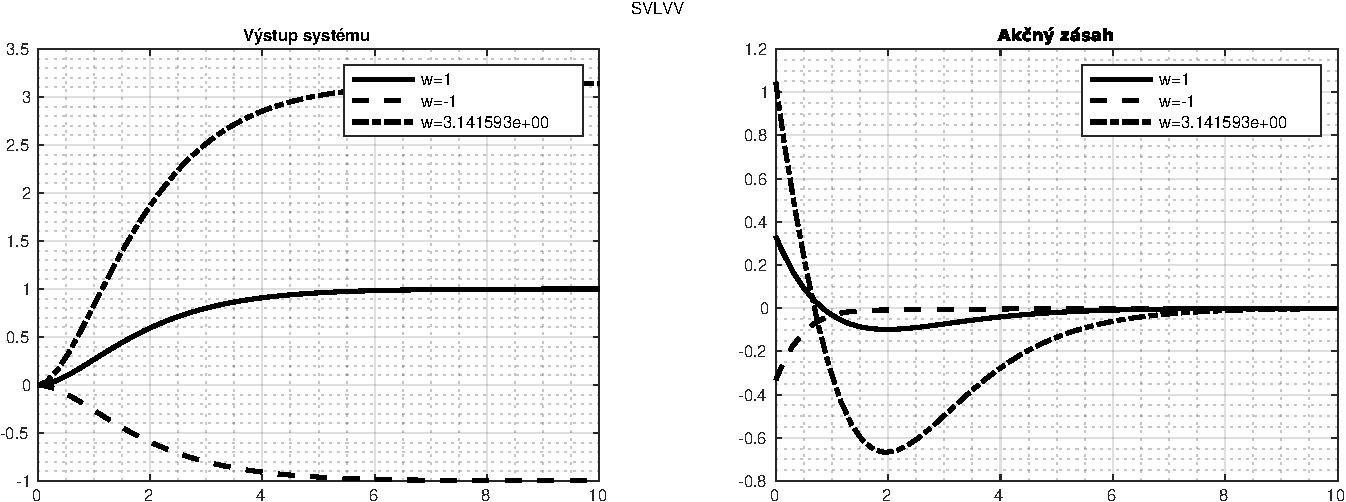
\includegraphics[width=\linewidth]{svlvvPr1/svlvvPr1Vysledok-crop}
		\caption{Regulácia výstupu na konštantnú hodnotu nelin. regulátorom navrhnutým pomocou metódy spätnoväzbovej linearizácie vstupno-výstupnej \cref{eqn:svlvvPr1SyavovyOpis}}
		\label{fig:svlvvPr1Vysledok}
	\end{figure}
	Pre porovnanie skúsme navrhnúť ešte regulátor pre tento systém, ktorý linearizujeme v rovnovažnom bode $x_1 = x_2 = 0$. Po linearizovaní bude mať systém tvar \cref{eqn:svlvvPr1LinearizovanySystem}. 
	\begin{equation}
	\begin{gathered}
	\Delta \dot{x_1}  = \Delta u \\
	\Delta \dot{x_2} = 3\Delta x_1 \\
	\Delta y = \Delta  x_2
	\end{gathered}
	\label{eqn:svlvvPr1LinearizovanySystem}
	\end{equation}
	Vyjadrime si prenosovú funkciu systému, pre jednoduchší návrh parametrov regulátora. Vyjadrenie prebieha v \cref{eqn:svlvvPr1VyjadreniePrenosuLinSys}. V tomto momente ešte potrebujeme zapojiť pred systém regulátor a vyjadriť prenos uzavretého regulačného obvodu.
	\begin{equation}
	\begin{aligned}
		\Delta  y &= \Delta x_2 = \frac{1}{s}  3 \Delta x_1 = \frac{1}{s^2}  3 \Delta u \\
		\implies \frac{\Delta y}{\Delta u } &= \frac{3}{s^2} \\
	\end{aligned}
	\label{eqn:svlvvPr1VyjadreniePrenosuLinSys}
	\end{equation}
	Zapojme na vstup systému PID regulátor, ako je na \cref{fig:svlvvPr1ZapojeinePIDNaLinSys}. Ktorý mý prenos \cref{eqn:svlvvPr1PIDPrenos}, kde $P, D, I$ sú parametre regulátora. Pre zjednodušenie ešte prenosy systému roznásobme, dostaneme tak prenos otvoreného obvodu $G_{ORO}$ daný \cref{eqn:svlvvPr1PIDPrenosORO}. 
	\begin{figure}[h!]
		\centering
		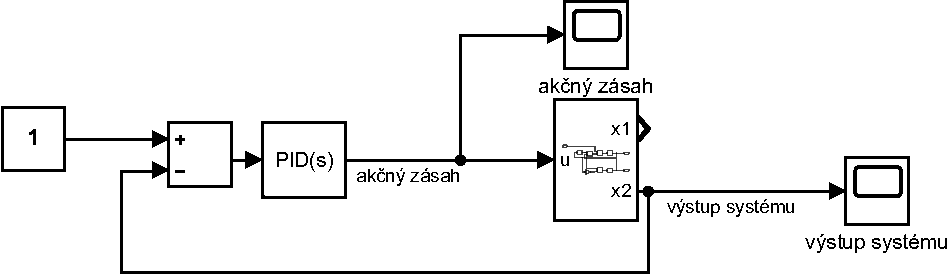
\includegraphics[width=0.8\linewidth]{svlvvPr1/svlvvPr1ZapojeniePID-crop}
		\caption{Zapojenie PID regulátora}
		\label{fig:svlvvPr1ZapojeinePIDNaLinSys}
	\end{figure}
	\begin{equation}
		\begin{aligned}
			\frac{U(s)}{E(s)} = P + Ds + \frac{I}{s} \\
		\end{aligned}
		\label{eqn:svlvvPr1PIDPrenos}
	\end{equation}
	\begin{equation}
	\begin{aligned}
	G_{ORO} = 3\frac{Ps + Ds^2 + I}{s^3} \\
	\end{aligned}
	\label{eqn:svlvvPr1PIDPrenosORO}
	\end{equation}
	Následne vyjadrime prenos uzavretého regulačného obvodu $G_{URO}$ podľa známeho pravidla zápornej spätnej väzby \cref{eqn:svlvvPr1PravidloZapornejSpantejVazby}. Dostaneme tak prenos \cref{eqn:svlvvPr1PrenosURO}.
	\begin{equation}
			\begin{aligned}
			G_{URO} = \frac{G_{ORO}}{1 + G_{ORO}}
			\end{aligned}
			\label{eqn:svlvvPr1PravidloZapornejSpantejVazby}
	\end{equation}
	\begin{equation}
		\begin{aligned}
		G_{URO} &= \frac{3\frac{Ps + Ds^2 + I}{s^3}}{1 + 3\frac{Ps + Ds^2 + I}{s^3}}  \\
		 		&= \frac{3(Ps + Ds^2 + I)}{s^3 + 3Ps + 3Ds^2 + 3I}
		\end{aligned}
		\label{eqn:svlvvPr1PrenosURO}
	\end{equation}
	Využime teraz metódu Pole-Placement na návrh parametrov regulátora, umiestnime póly na nasledovných pozíciách komplexnej roviny $p_1 = -5, p_2 = -4, p_3 = -3$. Teda nech sú póly reálne a záporné, čo zabezpečí stabilitu systému, keďže na kvalitu riadenia zatiaľ nekladieme dôraz.

	Polynóm ktorý bude mať zvolené korene, získame roznásobením polynmov prvého stupňa, ktorých korene sú zvolené póly, teda roznásobením \cref{eqn:svlvvPr1VznikZiadanehoPolynomu}. 
		\begin{equation}
	\begin{aligned}
	P(s) &= (s - p_1)(s - p_2)(s - p_3) \\
		 &= (s + 1)(s + 0.5)(s + 0.5) \\
		 &= s^3 + 2s^2 + 1.25s + 0.25\\
	\end{aligned}
	\label{eqn:svlvvPr1VznikZiadanehoPolynomu}
	\end{equation}
	Tento želaný polynóm porovnáme s CHPOLY URO, teda \cref{eqn:svlvvPr1Porovnanie}, dostaneme tak rovnice \cref{eqn:svlvvPr1RovniceParametrovPID} z ktorých vypočítame parametre regulátora.
	\begin{equation}
	\begin{aligned}
		s^3 + 2s^2 + 1.25s + 0.25= s^3 + 3Ps + 3Ds^2 + 3I\\
	\end{aligned}
	\label{eqn:svlvvPr1Porovnanie}
	\end{equation}
	\begin{equation}
	\begin{aligned}
		\begin{matrix}
		3P &= 2.00 \\
		3D &= 1.25 \\ 
		3I &= 0.25 \\
		\end{matrix}
		\implies 
		\begin{matrix}
		P &= \frac{2.00}{3} \\
		D &= \frac{1.25}{3} \\ 
		I &= \frac{0.25}{3}  \\
		\end{matrix}
	\end{aligned}
	\label{eqn:svlvvPr1RovniceParametrovPID}
	\end{equation}
	Skúsme tento regulátor aplikovať na nelineárny systém, ktorý chceme riadiť. Výsledok zo simulácie je na \cref{fig:svlvPr1VysledokPID}.
		\begin{figure}[h!]
			\centering
		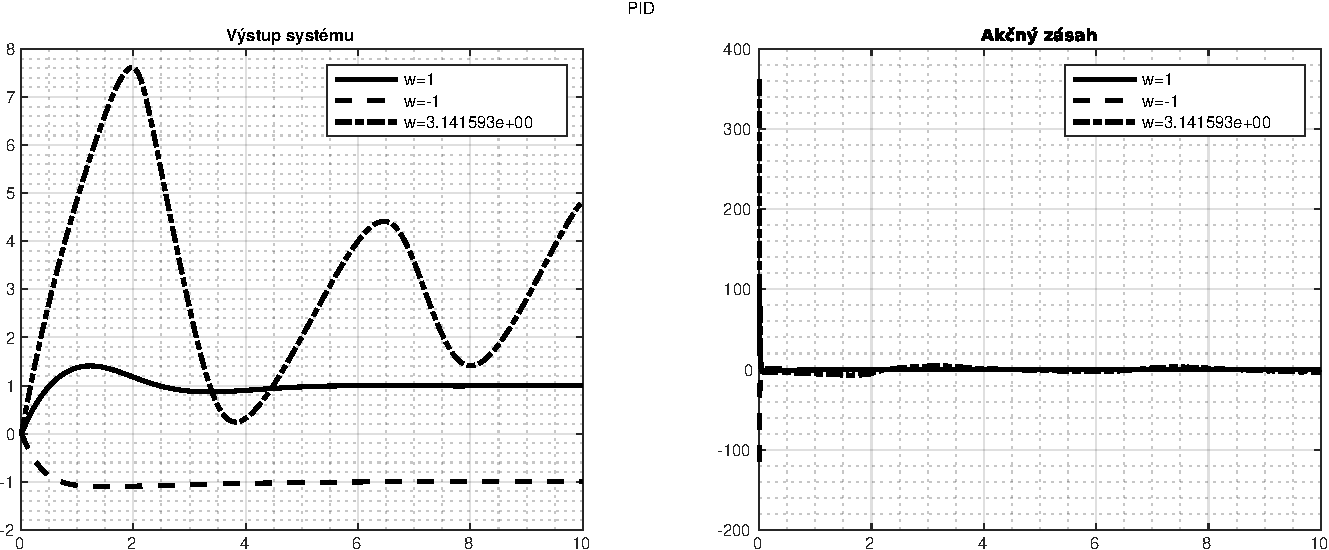
\includegraphics[width=\linewidth]{svlvvPr1/svlvvPr1PIDVysledok-crop}
		\caption{Regulácia výstupu na konštantnú hodnotu PID regulátorom navrhnutým pomocou metódy pole-placement}
		\label{fig:svlvPr1VysledokPID}
	\end{figure}
	Z tohto môžeme usúdiť, že nelineárne riadenie je v tomto prípade, nevyhnutné.
	
\end{document}
